%% preambolo

\documentclass[12pt, aspectratio=169, handout]{beamer}
\usepackage[utf8]{inputenc}
\usepackage[english, italian]{babel}
\usepackage[T1]{fontenc}
\usepackage{lmodern}
\usepackage{booktabs}
\usepackage{graphicx}
\usepackage{amsmath} 
\usepackage{amsthm}
\usepackage{amssymb}
\usepackage{siunitx}
\setbeamertemplate{navigation symbols}{} % nasconde icone navigazione nelle slide 
\setbeamercovered{invisible}
%%% fine preambolo


\title{\large Credit Risk Prediction With Statistical Learning:\\
	\large Comparing New Methods Using Italian Financial Reports}
\author{Marco Dodi}
\date{19 Ottobre 2026}
\institute{\normalsize Università degli Studi di Parma}

\begin{document}
	\maketitle
	
	% prima slide
	\begin{frame}{Campione e variabili input}
		\begin{itemize}
			\item<+-> Voci di bilancio sia da Stato Patrimoniale che Conto Economico per anni 2016, 2020, 2023: non indici di bilancio ma singole voci.
			\item<+-> Settori: inclusi i principali settori costituenti l'economia italiana (Edile, Manifattura, Ristorazione-Ricezione, Tessile)
			\item<+-> Forma Giuridica: solo società di capitali: quotate + non quotate
			\item<+-> \alert{Stato Giuridico}: Attiva Solvente, Attiva Insolvente, Fallita, Cessata (chiusura per fallimento) $\Rightarrow$ dummy $Y \in \left\{0, 1\right\}$
		\end{itemize}
	\end{frame}
	
	% 2 slide
	\begin{frame}{Regressione logistica penalità Lasso}
		La regressione logistica permette di stimare la probabilità di fallimento di una azienda. 
		\begin{block}{funzione obiettivo}
			$$\max_{\beta_{0}, \beta} \left\{\sum_{i = 1}^{N} \left[y_{i} \left(\beta_{0} + \beta^T x_{i}\right) - \log(1 + e^{\beta_{0} + \beta^T x_{i}})\right] - \alert{\lambda \sum_{j = 1}^{p} |\beta_{j}|}\right\}$$
		\end{block}
	\end{frame}
	
	% 3 slide
	\begin{frame}{Analisi discriminante}
		\begin{itemize}
			\item<+-> L'analisi discriminante propone un metodo alternativo per la stima della Probabilità di Default.
			\item<+-> La probabilità a posteriori può essere espressa in termini Bayesiani: $\Pr(Y = 1|X = x) = \frac{f_{k}(x) \pi_{k}}{\sum_{\ell = 1}^{K} f_{\ell}(x) \pi_{\ell}}$
			\item<+-> dove $f_k(x) = \frac{1}{(2\pi)^{p/2} |\boldsymbol{\Sigma}_{k}|^{1/2}} \exp\left[-\frac{1}{2} (x - \mu_{k})^T \boldsymbol{\Sigma}_{k}^{-1} (x - 	\mu_{k})\right]$
		\end{itemize}
	\end{frame}
	
	% 4 slide
	\begin{frame}{Distribuzione dei dati originali}
		\begin{columns}
			\begin{column}{0.50\textwidth}
				\centering
				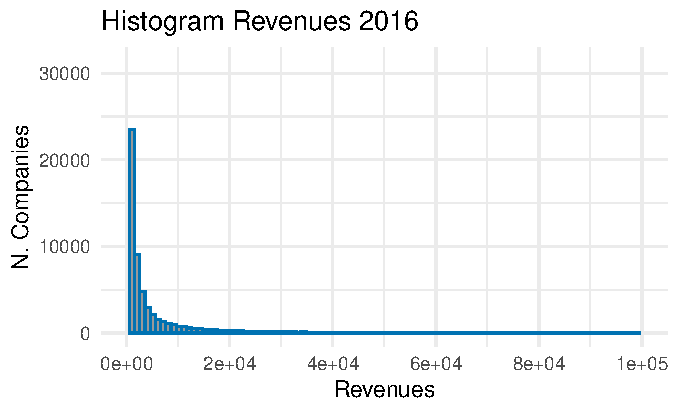
\includegraphics[width=\linewidth]{../graphics/pre-EDA/ist_raw_revenues_2016.pdf}
			\end{column}
			% seconda colonna
			\begin{column}{0.50\textwidth}
				\centering
				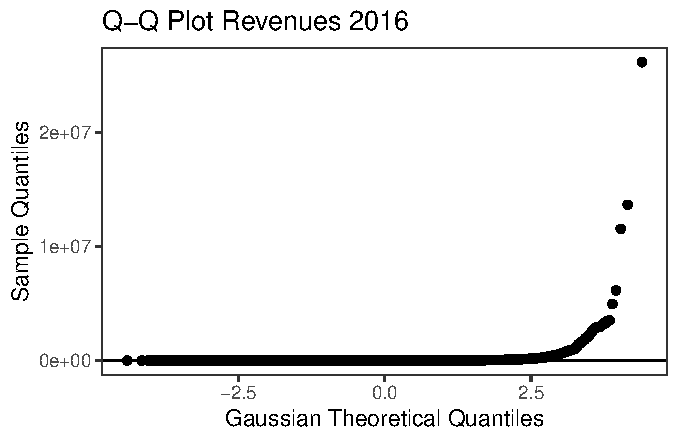
\includegraphics[width=\linewidth]{../graphics/pre-EDA/qqplot_raw_revenues_2016.pdf}
			\end{column}
		\end{columns}
		
		\bigskip
		
		Trasformazioni adottate: \textit{jittering} da una $U(0, 1)$, Yeo-Johnson, Box-Cox 
	\end{frame}
	
	% 5 
	\begin{frame}{Risultato trasformazioni}
		\centering
		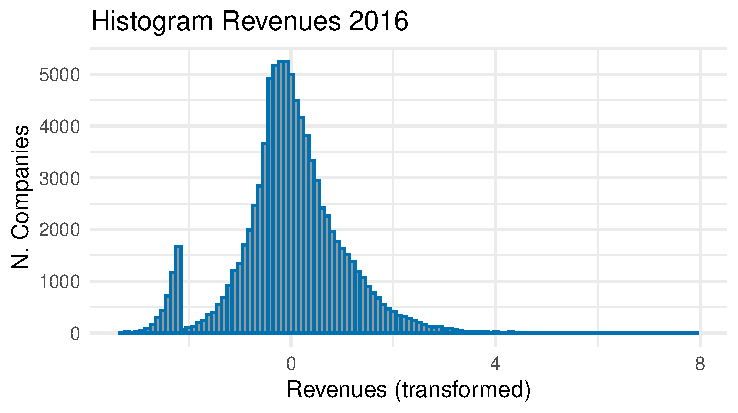
\includegraphics[width=0.48\textwidth, height=0.42\textheight]{figs/hist_rev_2016.pdf}
		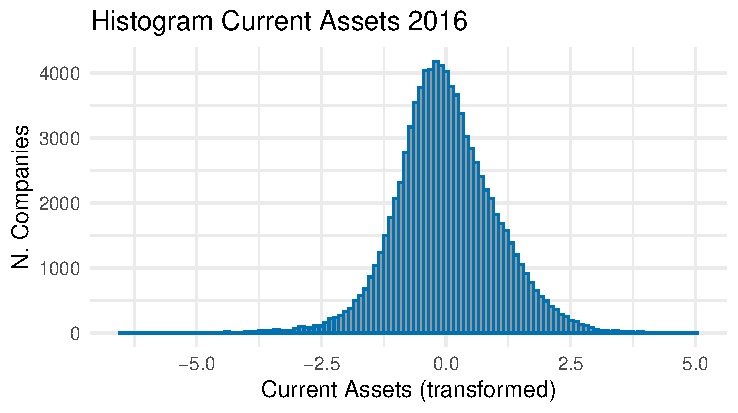
\includegraphics[width=0.48\textwidth, height=0.42\textheight]{figs/curr_asst_2016.pdf}
		
		\vspace{0.2cm}
		
		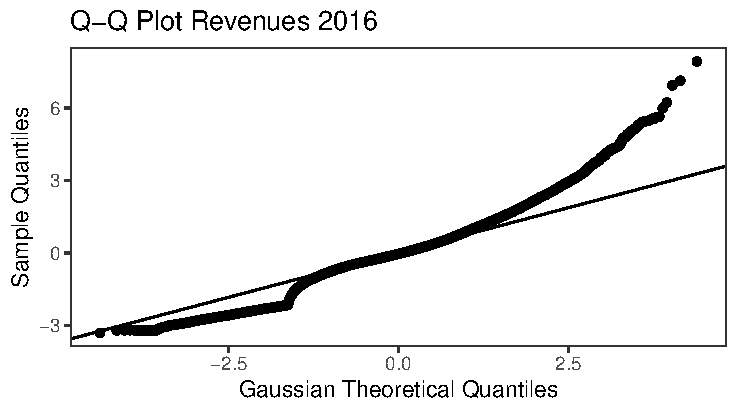
\includegraphics[width=0.48\textwidth, height=0.42\textheight]{figs/qqplot_rev_2016.pdf}
		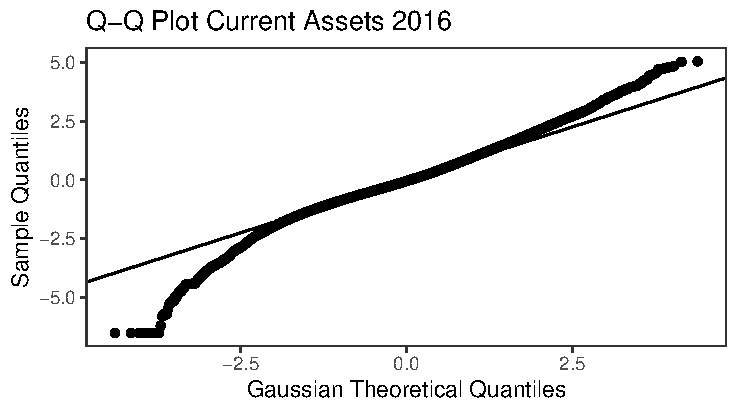
\includegraphics[width=0.48\textwidth, height=0.42\textheight]{figs/qqplot_curr_assets_2016.pdf}
	\end{frame}
	
	% 6 risultati lasso 2016
	\begin{frame}{Risultati Lasso logistico 2016}
		\begin{columns}[T]
			\begin{column}{0.65\textwidth}
				\centering
				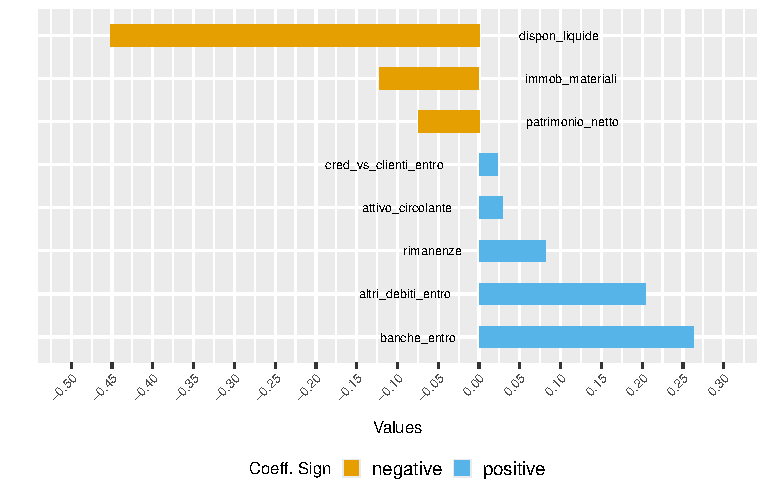
\includegraphics[width=\linewidth]{../results/logistic-lasso/lasso_coefficient_2016.pdf}
				
				\vspace{0.5cm}
				\footnotesize
				$\hat{\beta}_{\text{edile}} = 0.02833$,
			    $\hat{\beta}_{\text{tessile}} = 0.35323$
				
			\end{column}
			
			\begin{column}{0.35\textwidth}
				\centering
				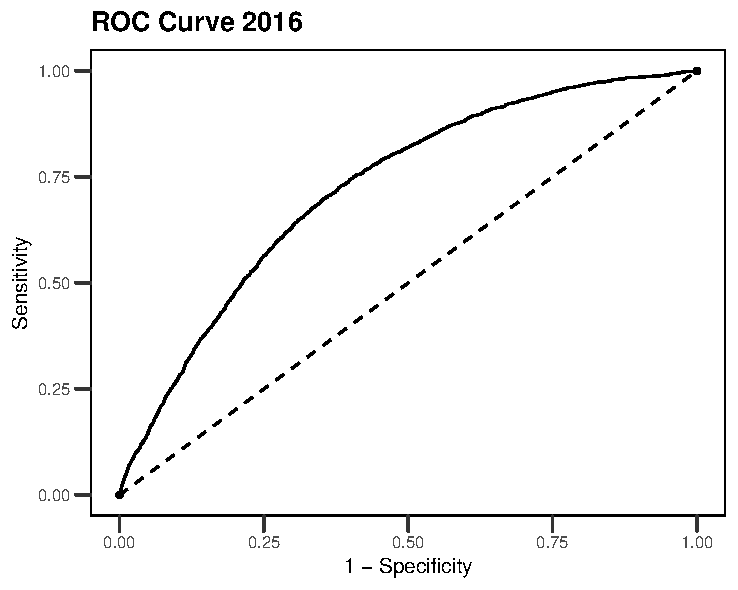
\includegraphics[width=\linewidth]{../results/logistic-lasso/lasso_roc_curve_2016.pdf}
				
				\vspace{0.1cm}
				\footnotesize
				AUC = 0.7247.
			\end{column}
		\end{columns}
	\end{frame}
	

% 7 risultati lasso 2020
\begin{frame}{Risultati Lasso logistico 2020}
	\begin{columns}[T]
		\begin{column}{0.65\textwidth}
			\centering
			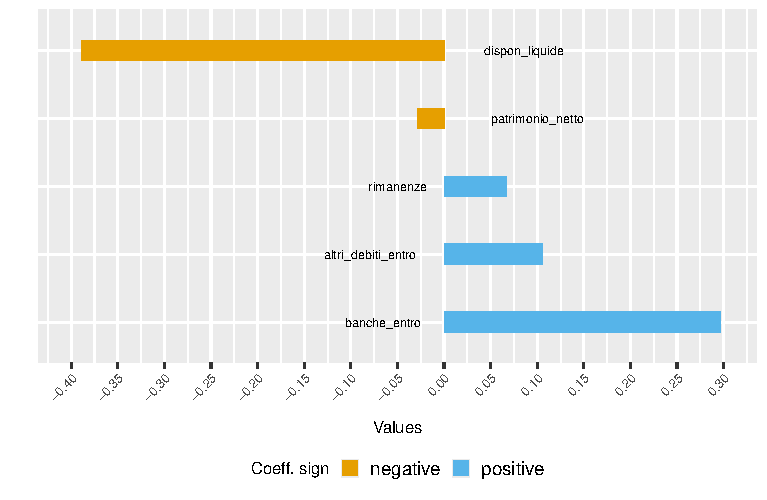
\includegraphics[width=\linewidth]{../results/logistic-lasso/lasso_coefficient_2020.pdf}
		\end{column}
		
		\begin{column}{0.35\textwidth}
			\centering
			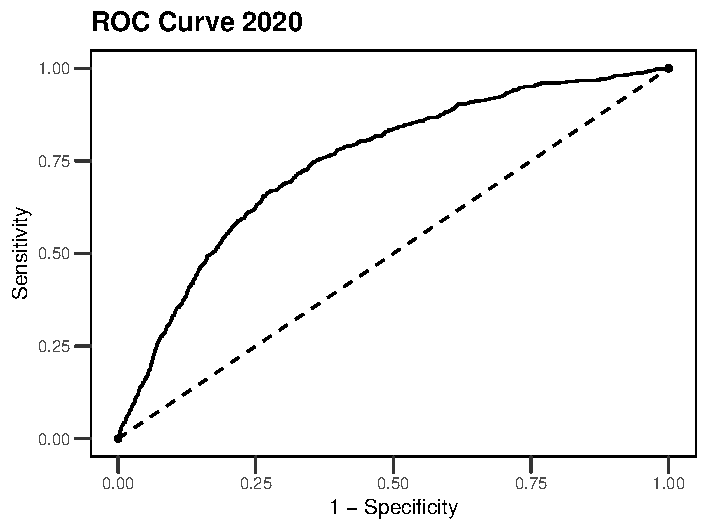
\includegraphics[width=\linewidth]{../results/logistic-lasso/lasso_roc_curve_2020.pdf}
			
			\vspace{0.2 cm}
			\footnotesize
			AUC = 0.7466.
		\end{column}
	\end{columns}
\end{frame}	

% 8 
\begin{frame}{Risultati Lasso logistico dati ricampionati 2023}
	\begin{columns}[T]
		\begin{column}{0.65\textwidth}
			\centering
			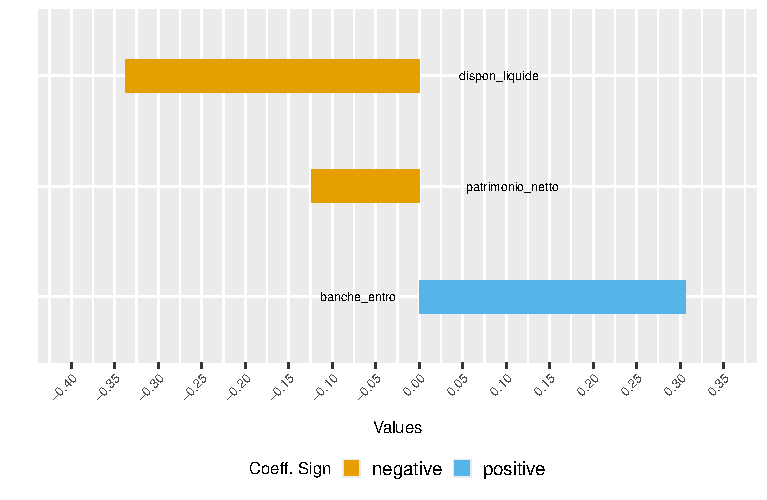
\includegraphics[width=\linewidth]{../results/logistic-lasso/lasso_sample_2023_coefficient.pdf}
		\end{column}
		
		\begin{column}{0.35\textwidth}
			\centering
			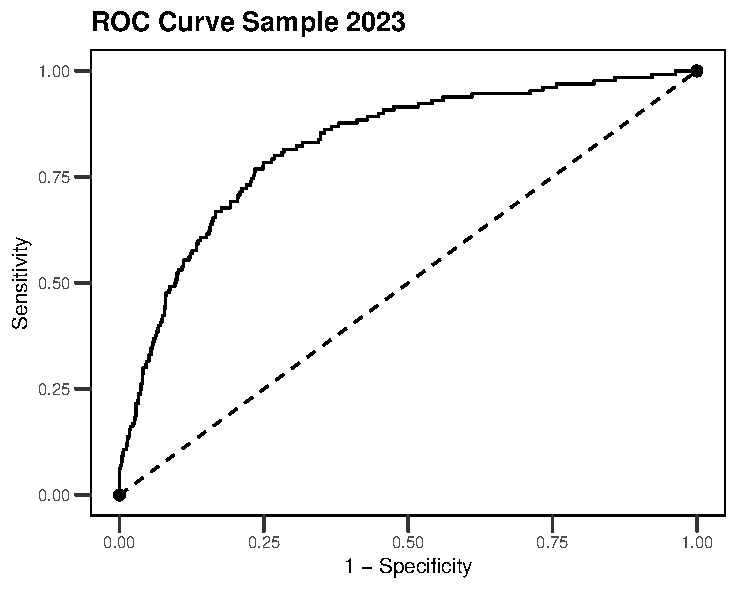
\includegraphics[width=\linewidth]{../results/logistic-lasso/lasso_roc_curve_sample_2023.pdf}
			
			\vspace{0.2 cm}
			\footnotesize
			AUC = 0.8248.
		\end{column}
	\end{columns}
\end{frame}

% 9
\begin{frame}{Risultati LDA 2016}
	\begin{columns}[T]
		\begin{column}{0.65\textwidth}
			\centering
			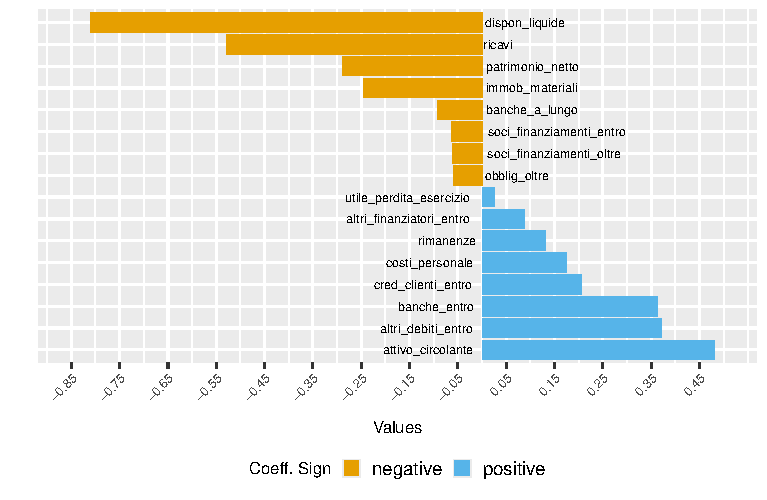
\includegraphics[width=\linewidth]{../results/lda/lda_2016_coefficient.pdf}
		\end{column}
		
		\begin{column}{0.35\textwidth}
			\centering
			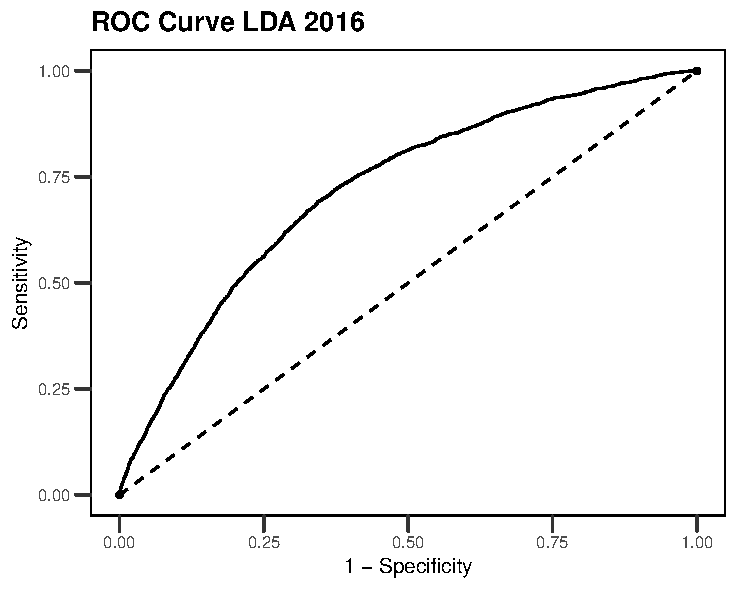
\includegraphics[width=\linewidth]{../results/lda/lda_roc_curve_2016.pdf}
			
			\vspace{0.2 cm}
			\footnotesize
			AUC = 0.7203.
		\end{column}
	\end{columns}
\end{frame}	
	
% 10
\begin{frame}{Risultati LDA 2020}
	\begin{columns}[T]
		\begin{column}{0.65\textwidth}
			\centering
			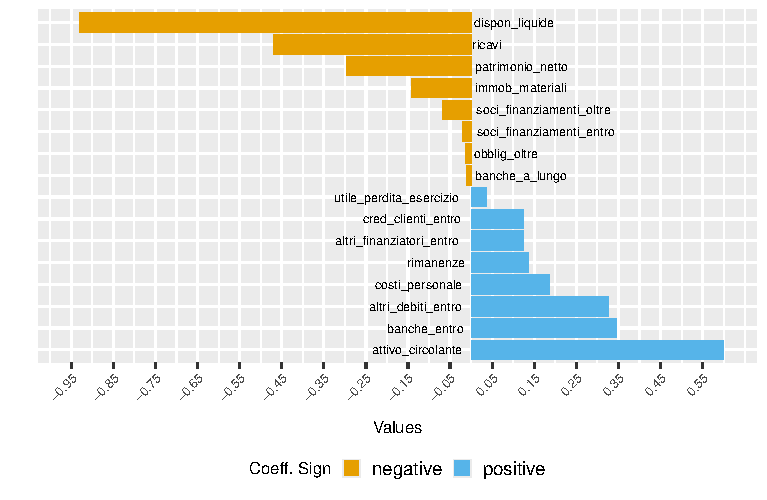
\includegraphics[width=\linewidth]{../results/lda/lda_2020_coefficient.pdf}
		\end{column}
		
		\begin{column}{0.35\textwidth}
			\centering
			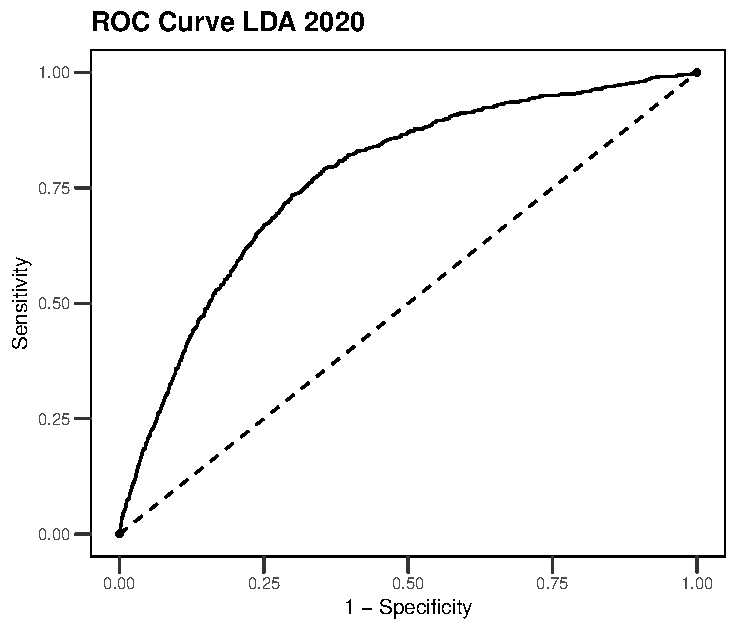
\includegraphics[width=\linewidth]{../results/lda/lda_roc_curve_2020.pdf}
			
			\vspace{0.2 cm}
			\footnotesize
			AUC = 0.7696
		\end{column}
	\end{columns}
\end{frame}
	
% 11
\begin{frame}{Risultati LDA 2023}
	\begin{columns}[T]
		\begin{column}{0.65\textwidth}
			\centering
			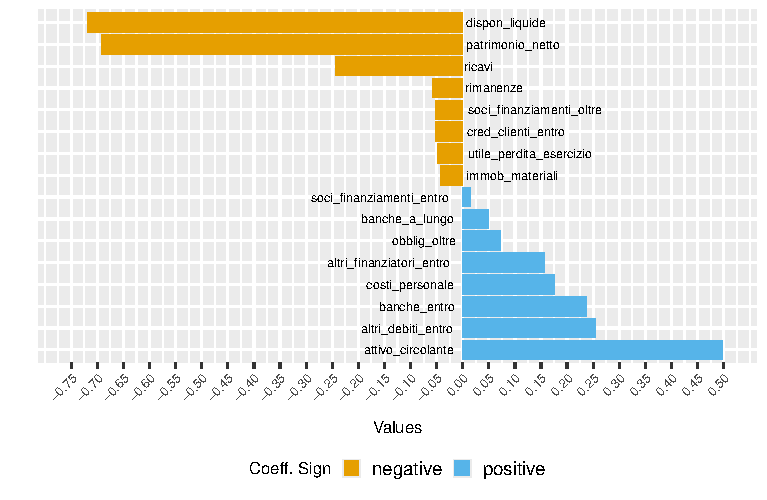
\includegraphics[width=\linewidth]{../results/lda/lda_2023_coefficient.pdf}
		\end{column}
		
		\begin{column}{0.35\textwidth}
			\centering
			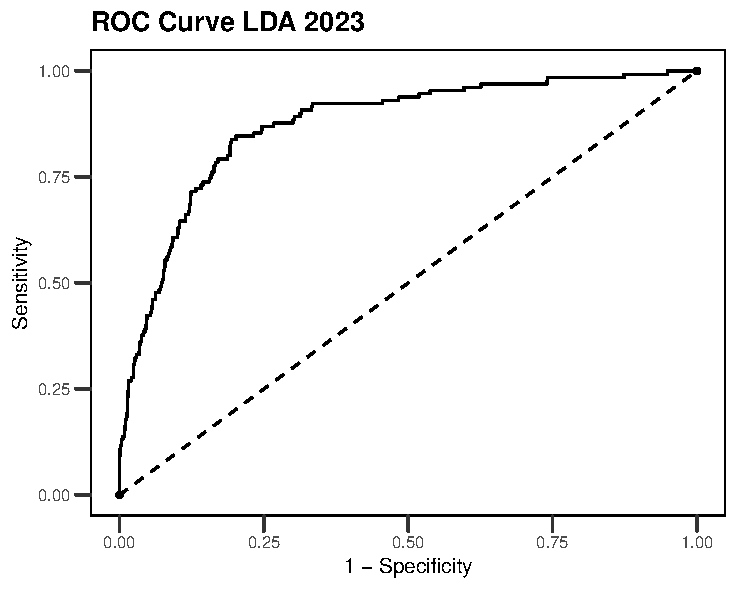
\includegraphics[width=\linewidth]{../results/lda/lda_roc_curve_2023.pdf}
			
			\vspace{0.2 cm}
			\footnotesize
			AUC = 0.8722
		\end{column}
	\end{columns}
\end{frame}
	
% 12
\begin{frame}{Risultati QDA e Alberi di classificazione}
	\begin{itemize}
		\item<+-> La QDA aggiunge un elemento di complessità ($\boldsymbol{\Sigma}_{k}$) $\rightarrow$ confini quadratici
		\item<+-> I risultati ottenuti tramite QDA sono i migliori: le matrici di covarianze diverse per le due classi permettono un miglior apprendimento dell'algoritmo
	\end{itemize}
	
	\vspace{0.5cm}
	\begin{itemize}
		\item<+-> La classificazione ad alberi hanno prodotto risultati insoddisfacenti: risentono dello sbilanciamento tra numero di imprese fallite e solventi + eterogeneità del campione
		\item<+-> Le curve ROC ricalcano la bisettrice che rappresenta la classificazione dettata dal caso
	\end{itemize}
\end{frame}
	
	

% saluti 
\begin{frame}
	\centering
	\huge
	Grazie per l'attenzione!
\end{frame}
	
\end{document}
